\chapter{\ifproject%
    \ifenglish Project Structure and Methodology\else โครงสร้างและขั้นตอนการทำงาน\fi
  \else%
    \ifenglish Project Structure\else โครงสร้างของโครงงาน\fi
  \fi
 }

ในบทนี้จะกล่าวถึงหลัการนําทฤษฎีที่เกี่ยวข้องมาประยุกต์ใช้ในการออกแบบ และพัฒนาระบบ


\makeatletter

% \renewcommand\section{\@startsection {section}{1}{\z@}%
%                                    {13.5ex \@plus -1ex \@minus -.2ex}%
%                                    {2.3ex \@plus.2ex}%
%                                    {\normalfont\large\bfseries}}

\makeatother
%\vspace{2ex}
% \titleformat{\section}{\normalfont\bfseries}{\thesection}{1em}{}
% \titlespacing*{\section}{0pt}{10ex}{0pt}
\section{โครงสร้างของระบบ}
% \ref{fig:Overall project structure}

% app -> streaming -> ci classify -> results -> Display -> add to cart -> payment -> order

\par ระบบจัดการการซื้อขายปลีกอัตโนมัติด้วยตนเอง โดยใช้เทคนิคความฉลาดเชิงคำนวณนั้นประกอบไปด้วยส่วนต่าง ๆ หลายส่วน เริ่มตั้งแต่ส่วนของแอปพลิเคชันบนโทรศัพท์มือถือ ที่จะถูกใช้งานโดยลูกค้าที่เข้ามาเลือกซื้อสินค้าในร้านค้า โดยมีจุดประสงค์หลักคือ การอำนวยความสะดวกให้ลูกค้าสามารถชำระสินค้าได้ด้วยตนเองโดยไม่ต้องผ่านจุดชำระเงินในร้าน ซึ่งการทำงานหลัก ๆ ของแอปพลิเคชันคือการให้ลูกค้าเลือกสินค้าลงตะกร้าเพื่อชำระเงิน นอกจากนี้ยังมีฟังก์ชันสำคัญในการจำแนกสินค้าผ่านการสตรีมมิ่ง ซึ่งอำนวยความสะดวกให้ลูกค้าสามารถหยิบสินค้าในร้าน แล้วแสกนรูปสินค้าเพื่อดูข้อมูลรายละเอียด หรือกดเข้าตะกร้าจ่ายเงินได้โดยไม่ต้องเลื่อนหาบนแอปพลิเคชันเอง โดยในการจำแนกประเภทสินค้านี้ จะมีการสื่อสารไปยังระบบให้บริการการจำแนกสินค้าซึ่งพัฒนาจากเทคนิคความฉลาดเชิงคำนวณ จากนั้นข้อมูลธุรกรรมต่าง ๆ ที่ลูกค้ากระทำบนแอปพลิเคชันจะถูกเก็บไว้บนฐานข้อมูลแบบคลาวด์ ซึ่งเป็นฐานข้อมูลที่ใช้ร่วมกันกับระบบเว็บไซต์สำหรับร้านค้า ทำให้เว็บไซต์ดังกล่าวสามารถนำข้อมูลการขายมาประมวลผล และแสดงให้ผู้ดูแลร้านค้าติดตามได้แบบเรียลไทม์ ในทางเดียวกันผู้ดูแลร้านค้าก็จะมีการจัดการเรื่องของข้อมูล และคลังสินค้าผ่านเว็บไชต์ร้านค้า ซึ่งข้อมูลดังกล่าวก็จะไปแสดงผลบนแอปพลิเคชันมือถือสำหรับลูกค้าเช่นกัน

โดยสรุปแล้ว ระบบจัดการการซื้อขายปลีกอัตโนมัติด้วยตนเอง โดยใช้เทคนิคความฉลาดเชิงคำนวณนั้นประกอบไปด้วยระบบ 4 ส่วนที่ทำงานร่วมกัน คือ 1. แอปพลิเคชันบนโทรศัพท์มือถือ (Mobile application)  2. ระบบให้บริการการจำแนกสินค้า (Classification Server) 3. ระบบฐานข้อมูล (Database) 4. เว็บไซต์สำหรับร้านค้า (Website Dashboard) โดยสามารถแสดงส่วนประกอบต่าง ๆ และการทำงานร่วมกันได้ ดังแผนภาพต่อไปนี้ \ref{fig:Overall project structure}



\begin{figure}[h]
  \begin{center}

    \vspace{0.5cm}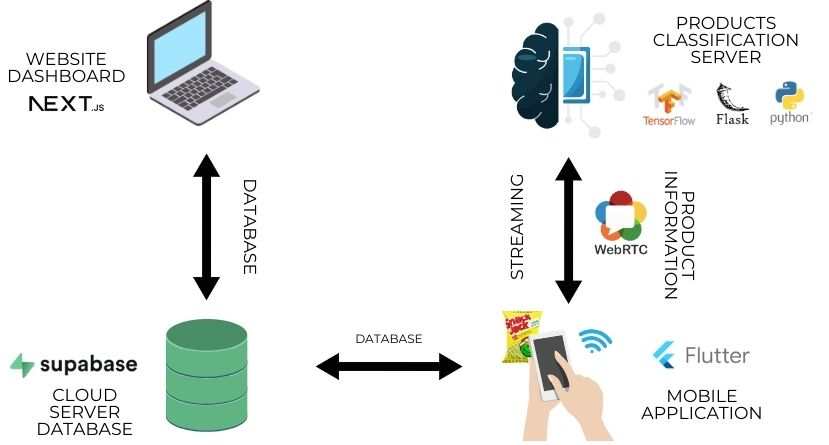
\includegraphics[scale=0.5]{pic/diagram/system_diagram.jpg}
  \end{center}

  \caption[Overall project structure]{Overall project structure}
  \label{fig:Overall project structure}
\end{figure}


\section{ระบบบริการจำแนกสินค้าผ่านรูปภาพ}
\subsection{เตรียมชุดข้อมูลฝึกสอน}
ข้อมูลที่ใช้ในการ train model ใช้รูปภาพจากสินค้าสินค้าจากห้อง 422  ทำการจัดเก็บข้อมูลรูปภาพ โดยใช้กล้องมือถือ
ในการถ่ายภาพโดยสินค้า 1 class (ชนิด) ทำการถ่ายภาพ 8 รูป ในมุมที่แตกต่างกัน
โดยโมเดลในโครงงานนี้จะใช้สินค้าทั้งหมด 51 class และเพิ่มอีก 1 class สำหรับพื้นหลัง (background class)
รวมเป็น 52 class
จัดเก็บใน Google Drive ดังรูป  \ref{fig:Google Drive} โดยทำการแยก รูปภาพตามหมวดหมู่ และทำการดึงข้อมูลมา train ผ่าน Google Colab
\begin{figure}[h]
  \begin{center}

    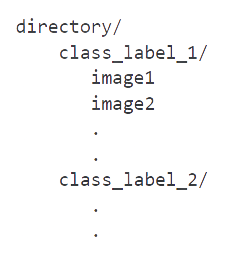
\includegraphics[scale=0.4]{pic/model/st.png}
  \end{center}

  \caption[Google Drive]{Google Drive}
  \label{fig:Google Drive}
\end{figure}
โดยในแต่ละรูป จะเป็นข้อมูล Array ขนาด 224x224x3

\subsection{K-Fold Cross Validation}

เพื่อตรวจสอบว่า model ที่เราทำการสร้าง ไม่ว่าจะเจอ dataset ที่ข้อมูลแตกต่างกันในแต่ละ fold ก็จะได้ accuracy ที่มีความใกล้เคียงในแต่ละ fold โดยที่ไม่แม่นยำแค่บาง dataset ซึ่งเป็นการ bias ต่อ dataset


\begin{center}
  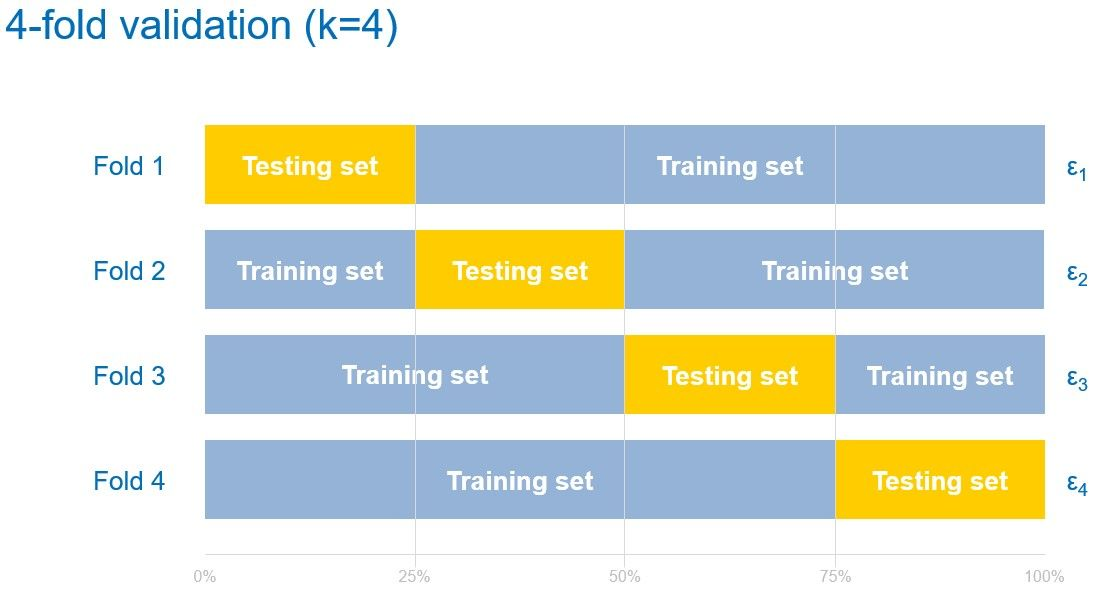
\includegraphics[scale=0.3]{pic/model/CrossValidation.png}\cite{CrossValidation}
\end{center}

ซึ่งในโครงงานนี้ ได้ทำการแบ่ง dataset เป็น ทั้งหมด 4 fold ดังรูป \ref{fig:Dataset}
โดยใน dataset แต่ละ fold ก็จะทำการ augmentation เพื่อเพิ่มจำนวนข้อมูลที่ใช้ในการ train model ของแต่ละ fold
\begin{figure}[h]
  \begin{center}

    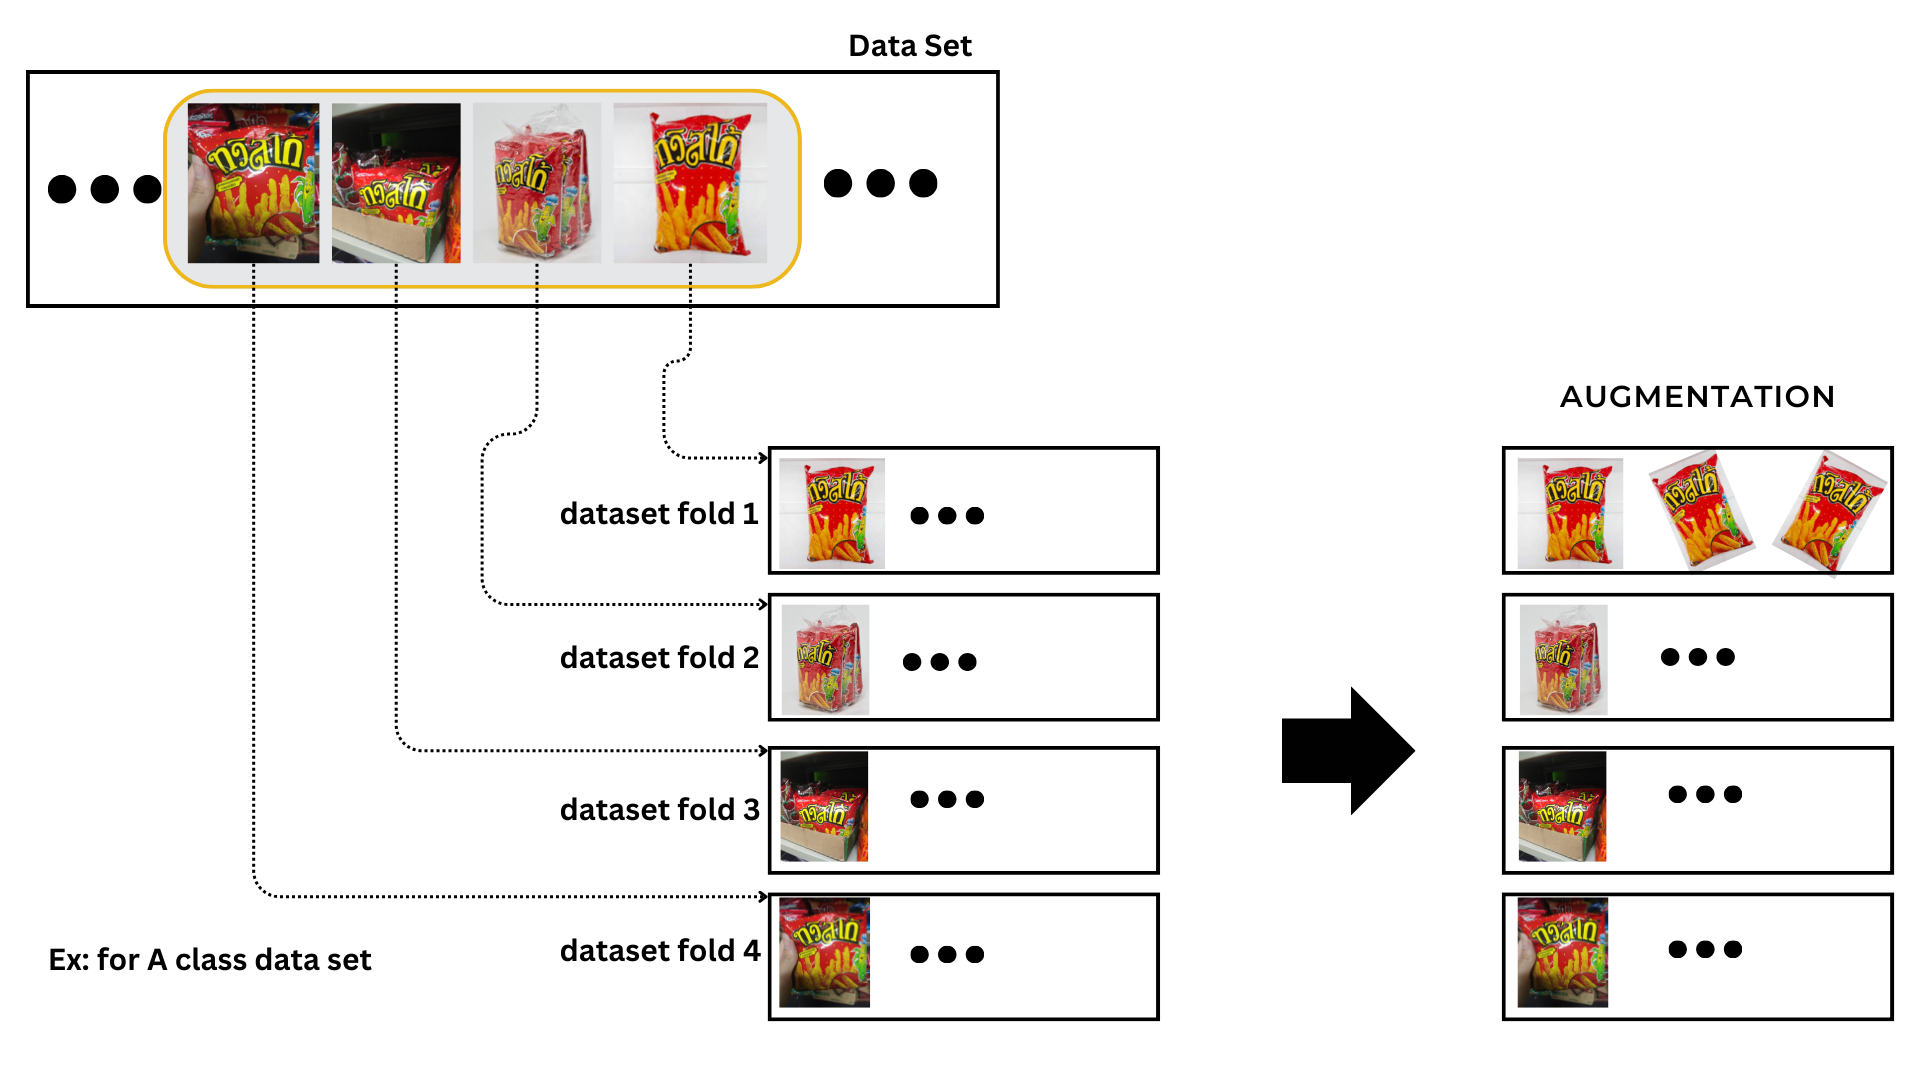
\includegraphics[scale=0.25]{pic/model/fold_aug.png}
  \end{center}

  \caption[Dataset]{Dataset}
  \label{fig:Dataset}
\end{figure}

\newpage



\subsection{Data augmentation การเพิ่ม traing data}
เพื่อให้มี train dataset ในจำนวนมาก
โดยในแต่ละ 1 รูปภาพที่ถ่าย ซึ่งเป็นรูปภาพ RGB ขนาด 224x224 pixel
นำไปสร้างเป็นรูปภาพใหม่ โดยใช้วิธีการ หมุน และ กลับด้าน ด้วยมุม -20,-15,-10,-5,0,5,10,15,20 องศา
โดย 1 รูปภาพผ่านการ generate datasets จะกลายเป็น 18 รูปภาพซึ่งมีความแตกต่างกันเล็กน้อย ตามรูป \ref{fig:Dataset generator}

\begin{figure}[h]
  \begin{center}

    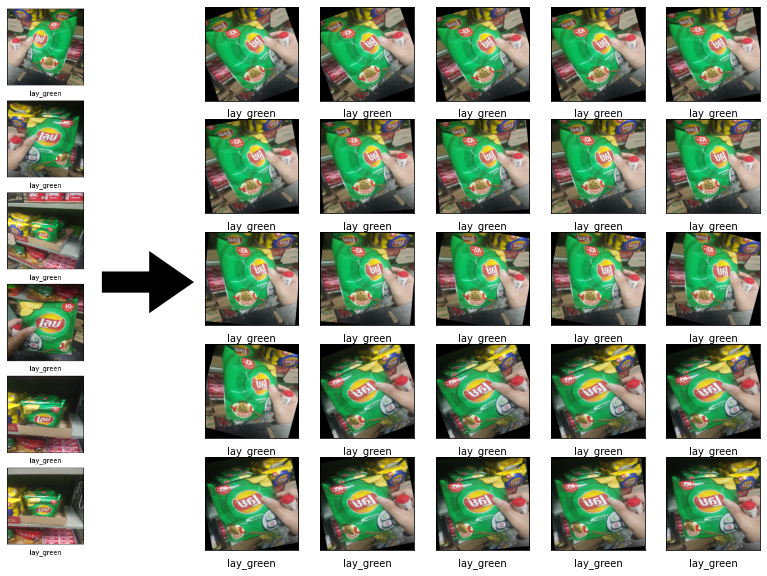
\includegraphics[scale=0.4]{pic/model/lay_genmore.png}
  \end{center}

  \caption[Dataset generator]{Dataset generator}
  \label{fig:Dataset generator}
\end{figure}




\newpage
\subsection{Model Architecture}
โดยโมเดลในโครงงานนี้จะใช้ Xception pre-trained ซึ่งเป็น Convolutional Neural Network ซึ่งมีความลึก 71 layers.
เป็นโมเดลที่ผ่านการจากรูปภาพต่าง ๆ มากกว่าล้านรูปภาพจาก ImageNet database .
ซึ่งจะมีโครงสร้างดังรูป


\begin{center}
  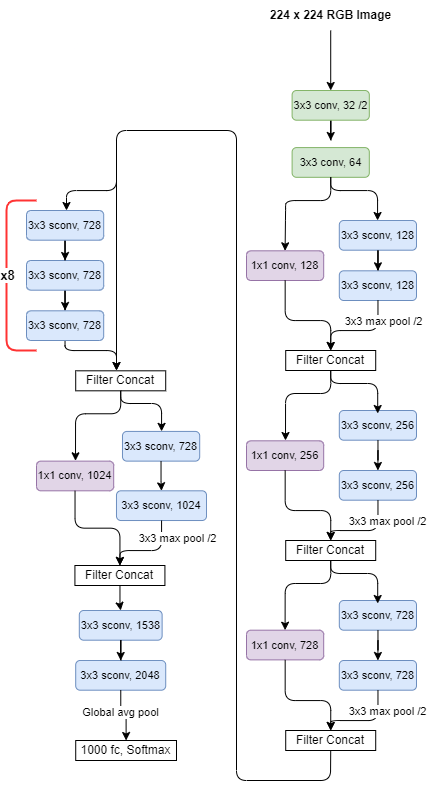
\includegraphics[scale=0.35]{pic/model/x_1.png}\cite{Xception}
\end{center}


โดยการนำ Xception model มาใช้ในการแยกคุณลักษณะเด่นของรูปภาพ  และ สร้างโมเดลมาต่อท้ายเพื่อ
เรียนรู้ลักษณะเด่นจากที่ Xception ทำการแยกออกมาได้

โดยโครงสร้างของ model จะเป็นดังรูป \ref{fig:Classification model}
% transfer learning - Xceptionโดย pre-train 'Xception' model 

\begin{figure}[h]
  \begin{center}

    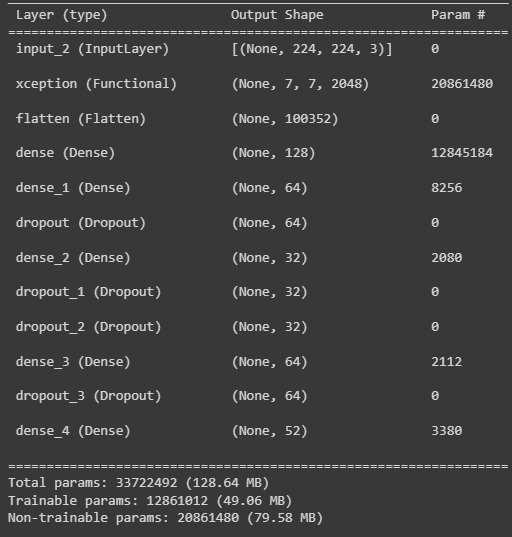
\includegraphics[scale=0.6]{pic/model/model.png}

  \end{center}

  \caption[Classification model]{Classification model}
  \label{fig:Classification model}
\end{figure}

 

ซึ่ง model ที่จะใช้ก็จะเป็น Xception model ที่รับ Input ขนาด 224 x 224 x 3 ตามขนาดรูปภาพ 224x224 pixel และตาม layer RGB

โดย Xception เป็น model ตั้งต้นที่่ผ่าน pre train model จะทำหน้าที่เป็น feature extraction  ลักษณะเด่นของรูปภาพ
โดย Xception จะถูก lock ค่าของ weight เอาไว้เพื่อไม่ไห้ค่าของ weight ที่ได้เรียนรู้ข้อมูลมาจาก ImageNet หายไป
ซึ่ง exercitation มี weight ทั้งหมด 20 ล้าน parameter

และนำ layer มาต่อท้าย model ด้วย fully connected node ที่เรียกว่า Dense layer จำนวน 128 , 64 , 32 ,  64 node และ
layer สุดท้าย ซึ่งมีขนาดเท่ากับจำนวน class ของสินค้า ซึ่งทำหน้าที่เป็น classifier
โดย Dense layer ซึ่งเชื่อมกันแบบ fully connected ที่สามารถ เรียนรู้และปรับค่าของ weight ได้
ในโครงสร้างทดสอบนี้จะมี weight ที่่สามารถเรียนรู้ หรือ เปลี่ยนแปลงได้ 12 ล้าน parameters


\subsection{classification products}
จากรูปภาพใน 52 class ผ่านการ generate datasets จะมี dataset ทั้งหมด 4432 sample ต่อ 1 Fold
ทำการแบ่งเป็น train 3546 sample และ  886 sample สำหรับการ evaluate
โดยจาก train 3546 แบ่ง 50\% สำหรับการ validation ในระหว่างการ train model

สำหรับเป็น service ในการ classify products ของ application ผ่าน aiortc  และเว็บ WebSocket



\newpage

\section{ระบบแอปพลิเคชันสำหรับโทรศัพท์มือถือ}
\subsection{ขอบเขตการพัฒนาระบบแอปพลิเคชันสำหรับโทรศัพท์มือถือ}
\begin{enumerate}
  \item ผู้คนทั่วไปสามารถลงทะเบียนเข้าใช้งานได้
  \item สามารถใช้กล้องโทรศัพท์มือถือแสกนสินค้าเพื่อสตรีมภาพระบบบริการจำแนกสินค้า (Classification server) เพื่อจำแนกสินค้าที่แสกน แล้วแสดงผล บนแอปพลิเคชัน
  \item สามารถดูรายการสินค้าทั้งหมดในร้านได้
  \item สามารถกดดูข้อมูลสินค้าที่เลือก หรือแสกนได้
  \item สามารถเพิ่มหรือลดสินค้าในตะกร้าได้
  \item สามารเติมเงินเป็นเครดิตในแอปพลิเคชันได้
  \item สามารถชําระสินค้าผ่านเครดิตเงินเติมในตัวแอปพลิเคชัน

\end{enumerate}

\subsection{การออกแบบระบบแอปพลิเคชันสำหรับโทรศัพท์มือถือ}
สำหรับระบบแอปพลิเคชันสำหรับโทรศัพท์มือถือนั้น ได้ออกแบบให้เป็นแอปพลิเคชันที่ให้บริการบนระบบปฏิบัติการแอนดรอยด์ ทำการพัฒนาโดยใช้ Flutter ร่วมกับ Supabase ในการเชื่อมต่อกับฐานข้อมูลที่ได้เตรียมไว้ รวมถึงใช้ในการทำระบบยืนยันตัวตน ลูกค้าทั่วไปสามารถติดตั้งแอปพลิเคชันบนโทรศัพท์มือถือ และลงทะเบียนใช้งาน เพื่อนำมาใช้ซื้อสินค้าในร้านด้วยตนเอง ผ่านการกดเลือกสินค้าในรายการ หรือแสกนสินค้าจริง ซึ่งระบบจะจำแนกสินค้าได้ผ่านการถ่ายทอดสด โดยมีการใช้บริการผ่าน WebSocket ซึ่งติดต่อกับระบบบริการจำแนกสินค้า (Classification server) ที่ได้ทำการฝึกสอนไว้แล้ว จากนั้นจะมีการเชื่อมต่อกับฐานข้อมูลแล้วตอบกลับมายังแอพลิเคชันเพื่อแสดงผลให้กับผู้ใช้งาน ซึ่งหน้าการใช้งานทั้งหมดของแอปพลิเคชัน ประกอบไปด้วย

\begin{enumerate}
  \item หน้าลงทะเบียน และลงชื่อเข้าใช้งาน (login \& Register)
  \item หน้าโปรไฟล์ผู้ใช้งาน และหน้าประวัติการซื้อสินค้า (Profile \& Purchase History)
  \item หน้าแก้ไขโปรไฟล์ผู้ใช้งาน และเติมเงิน (Edit Profile \& Credit Topup)
  \item หน้าแสดงรายการสินค้า (Stock)
  \item หน้าแสดงข้อมูลสินค้า (Product Details)
  \item หน้าตะกร้าสินค้า และจ่ายเงิน (Cart \& Checkout)

\end{enumerate}

\subsubsection{Use Case}
\newpage
\ref{fig:Mobile Application Use Case Diagram}

\begin{figure}[h]
  \begin{center}

    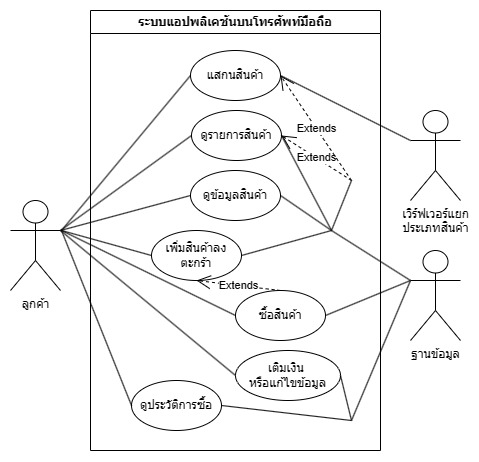
\includegraphics[scale=0.5]{pic/diagram/usecase-mobile.jpg}
  \end{center}

  \caption[Dataset generator]{Dataset generator}
  \label{fig:Mobile Application Use Case Diagram}
\end{figure}

\begin{table}[htbp]
  \centering
  \caption{แสดงการอธิบายกรณีการใช้งานกรณีแสกนสินค้าของระบบแอปพลิเคชันสำหรับโทรศัพท์มือถือ}
  \label{tab:example}
  \begin{tabularx}{\textwidth}{|p{3cm}|X|}
    \hline
    \multirow{1}{3cm}{Use Case ID:}      & 1                                                             \\
    \hline
    \multirow{1}{3cm}{Use Case Name:}    & แสกนสินค้า                                                      \\
    \hline
    \multirow{1}{3cm}{Actor:}            & 1. ผู้ใช้งานแอปพลิเคชัน 2. ฐานข้อมูล 3. ระบบบริการจำแนกสินค้า            \\
    \hline
    \multirow{2}{3cm}{Pre-Condition:}    & 1. เข้าสู่ระบบ                                                   \\ & 2. ระบบจำแนกสินค้าเปิดให้บริการ\\
    \hline
    \multirow{1}{3cm}{Post-Condition:}   & สินค้าที่แสกนแสดงผลบนแอปพลิเคชัน                                    \\
    \hline
    \multirow{3}{3cm}{Event flow:}       & 1. กดเมนูแสกนสินค้า                                              \\
                                         & 2. เชื่อมต่อระบบบริการจำแนกสินค้า                                    \\ & 3.  ลูกค้าส่องกล้องมือถือไปที่สินค้า \\
                                         & 4. ดึงข้อมูลจากฐานข้อมูล                                           \\
                                         & 5. ระบบแสดงสินค้าที่แสกนบนแอปพลิเคชัน                               \\
    \hline
    \multirow{1}{3cm}{Alternative flow:} & 5. หากไม่ใช่สินค้าที่ขายในร้าน ระบบจะแจ้งเตือนว่าไม่มีข้อมูลสินค้าที่แสกนในระบบ \\
    \hline
  \end{tabularx}
\end{table}

\begin{table}[htbp]
  \centering
  \caption{แสดงการอธิบายกรณีการใช้งานกรณีดูรายการสินค้าของระบบแอปพลิเคชันสำหรับโทรศัพท์มือถือ}
  \label{tab:example}
  \begin{tabularx}{\textwidth}{|p{3cm}|X|}
    \hline
    \multirow{1}{3cm}{Use Case ID:}      & 2                              \\
    \hline
    \multirow{1}{3cm}{Use Case Name:}    & ดูรายการสินค้า                    \\
    \hline
    \multirow{1}{3cm}{Actor:}            & 1. ผู้ใช้งานแอปพลิเคชัน 2. ฐานข้อมูล  \\
    \hline
    \multirow{1}{3cm}{Pre-Condition:}    & เข้าสู่ระบบ                       \\
    \hline
    \multirow{1}{3cm}{Post-Condition:}   & ลูกค้าสามารถดูรายการสินค้าที่มีในร้านได้ \\
    \hline
    \multirow{3}{3cm}{Event flow:}       & 1. กดเมนูรายการสินค้า             \\
                                         & 2. ดึงข้อมูลจากฐานข้อมูล            \\ & 3. แสดงรายการสินค้าพร้อมจำนวนในคลัง \\
    \hline
    \multirow{1}{3cm}{Alternative flow:} & -                              \\
    \hline
  \end{tabularx}
\end{table}

\begin{table}[htbp]
  \centering
  \caption{แสดงการอธิบายกรณีการใช้งานกรณีดูข้อมูลสินค้าของระบบแอปพลิเคชันสำหรับโทรศัพท์มือถือ}
  \label{tab:example}
  \begin{tabularx}{\textwidth}{|p{3cm}|X|}
    \hline
    \multirow{1}{3cm}{Use Case ID:}      & 3                                           \\
    \hline
    \multirow{1}{3cm}{Use Case Name:}    & ดูข้อมูลสินค้า                                   \\
    \hline
    \multirow{1}{3cm}{Actor:}            & 1. ผู้ใช้งานแอปพลิเคชัน 2. ฐานข้อมูล               \\
    \hline
    \multirow{3}{3cm}{Pre-Condition:}    & 1. เข้าสู่ระบบ                                 \\ & 2.1 กดเมนูรายการสินค้า แล้วกดเลือกสินค้าที่ต้องการ \\
                                         & 2.2 กดเมนูแสกนสินค้า แล้วแสกนสินค้าสำเร็จ           \\
    \hline
    \multirow{1}{3cm}{Post-Condition:}   & แสดงหน้าต่างรายละเอียดข้อมูลของสินค้าที่เลือก หรือแสกน \\
    \hline
    \multirow{3}{3cm}{Event flow:}       & 1. กดปุ่มดูรายละเอียดข้อมูล                       \\
                                         & 2. แสดงข้อมูล                                 \\
    \hline
    \multirow{1}{3cm}{Alternative flow:} & 2. ไม่พบข้อมูลรายละเอียดของสินค้าในฐานข้อมูล        \\
    \hline
  \end{tabularx}
\end{table}

\begin{table}[htbp]
  \centering
  \caption{แสดงการอธิบายกรณีการใช้งานกรณีเพิ่มสินค้าลงตะกร้าของระบบแอปพลิเคชันสำหรับโทรศัพท์มือถือ}
  \label{tab:example}
  \begin{tabularx}{\textwidth}{|p{3cm}|X|}
    \hline
    \multirow{1}{3cm}{Use Case ID:}      & 4                                           \\
    \hline
    \multirow{1}{3cm}{Use Case Name:}    & เพิ่มสินค้าลงตะกร้า                              \\
    \hline
    \multirow{1}{3cm}{Actor:}            & 1. ผู้ใช้งานแอปพลิเคชัน 2. ฐานข้อมูล               \\
    \hline
    \multirow{3}{3cm}{Pre-Condition:}    & 1. เข้าสู่ระบบ                                 \\ & 2.1 กดเมนูรายการสินค้า แล้วกดเลือกสินค้าที่ต้องการ \\
                                         & 2.2 กดเมนูแสกนสินค้า แล้วแสกนสินค้าสำเร็จ           \\
    \hline
    \multirow{1}{3cm}{Post-Condition:}   & แสดงหน้าต่างรายละเอียดข้อมูลของสินค้าที่เลือก หรือแสกน \\
    \hline
    \multirow{3}{3cm}{Event flow:}       & 1. เลือกจำนวนที่ต้องการซื้อ                        \\
                                         & 2. กดปุ่มตะกร้า                                \\ & 3. ระบบเพิ่มสินค้า ในจำนวนที่เลือกเข้าตะกร้า \\
    \hline
    \multirow{1}{3cm}{Alternative flow:} & -                                           \\
    \hline
  \end{tabularx}
\end{table}

\begin{table}[htbp]
  \centering
  \caption{แสดงการอธิบายกรณีการใช้งานกรณีเพิ่มสินค้าลงตะกร้าของระบบแอปพลิเคชันสำหรับโทรศัพท์มือถือ}
  \label{tab:example}
  \begin{tabularx}{\textwidth}{|p{3cm}|X|}
      \hline
      \multirow{1}{3cm}{Use Case ID:} & 5 \\
      \hline
      \multirow{1}{3cm}{Use Case Name:} & ซื้อสินค้า \\
      \hline
      \multirow{1}{3cm}{Actor:} & 1. ผู้ใช้งานแอปพลิเคชัน 2. ฐานข้อมูล \\
      \hline
      \multirow{2}{3cm}{Pre-Condition:} & 1. เข้าสู่ระบบ \\ & 22. มีสินค้าอย่างน้อย 1 ชิ้นในตะกร้า \\
      \hline
      \multirow{1}{3cm}{Post-Condition:} & ลูกค้าซื้อสินค้าสำเร็จ ระบบตัดเงินเครดิตของลูกค้า และเก็บรายการสินค้าที่ซื้อในประวัติการซื้อสินค้า \\
      \hline
      \multirow{3}{3cm}{Event flow:} & 1. เลือกเมนู Cart \\ 
      & 2. เช็คสินค้าในตะกร้าว่าถูกต้องตามที่ต้องการหรือไม่ \\ & 3. กดปุ่มซื้อสินค้า \\
      & 4. บันทึก และแก้ไขข้อมูลบนฐานข้อมูล \\ & 5. แสดงผลการซื้อสินค้าสำเร็จ \\
      \hline
      \multirow{5}{3cm}{Alternative flow:} & \textbf{กรณีที่ 1: หากต้องการลบสินค้าในตะกร้า} \\ 
      & 2. เช็คสินค้าในตะกร้าว่าถูกต้องตามที่ต้องการหรือไม่ \\ & \textbf{กรณีที่ 2: หากสินค้าในคลังไม่พอจำนวนที่ซื้อ หรือหมด} \\
      & 4. เช็คจำนวนสินค้าที่มีบนฐานข้อมูลไม่พอกับที่ต้องการซื้อ \\ & 5. แสดงผลการซื้อสินค้าไม่สำเร็จ \\
      \hline
  \end{tabularx}
\end{table}


\begin{table}[htbp]
  \centering
  \caption{แสดงการอธิบายกรณีการใช้งานกรณีเพิ่มสินค้าลงตะกร้าของระบบแอปพลิเคชันสำหรับโทรศัพท์มือถือ}
  \label{tab:example}
  \begin{tabularx}{\textwidth}{|p{3cm}|X|}
      \hline
      \multirow{1}{3cm}{Use Case ID:} & 6 \\
      \hline
      \multirow{1}{3cm}{Use Case Name:} & ดูประวัติการซื้อสินค้า \\
      \hline
      \multirow{1}{3cm}{Actor:} & 1. ผู้ใช้งานแอปพลิเคชัน 2. ฐานข้อมูล \\
      \hline
      \multirow{1}{3cm}{Pre-Condition:} & เข้าสู่ระบบ \\ 
      \hline
      \multirow{1}{3cm}{Post-Condition:} & ลูกค้ารับรู้ข้อมูลผู้ใช้งาน และรายการสินค้าที่เคยซื้อ \\
      \hline
      \multirow{3}{3cm}{Event flow:} & 1. กดที่ชื่อผู้ใช้งาน \\ 
      & 2. เข้าสู้หน้าโปรไฟล์ผู้ใช้งาน \\ & 3. แสดงชื่อผู้ใช้ เครดิตเงินเติม และรายการประวัติสินค้าที่เคยซื้อ \\
      \hline
      \multirow{1}{3cm}{Alternative flow:} & - \\
      \hline
  \end{tabularx}
\end{table}

\begin{table}[htbp]
  \centering
  \caption{แสดงการอธิบายกรณีการใช้งานกรณีเพิ่มสินค้าลงตะกร้าของระบบแอปพลิเคชันสำหรับโทรศัพท์มือถือ}
  \label{tab:example}
  \begin{tabularx}{\textwidth}{|p{3cm}|X|}
      \hline
      \multirow{1}{3cm}{Use Case ID:} & 7 \\
      \hline
      \multirow{1}{3cm}{Use Case Name:} & เติมเงิน และแก้ไขข้อมูล \\
      \hline
      \multirow{1}{3cm}{Actor:} & 1. ผู้ใช้งานแอปพลิเคชัน 2. ฐานข้อมูล \\
      \hline
      \multirow{1}{3cm}{Pre-Condition:} & เข้าสู่ระบบ \\ 
      \hline
      \multirow{1}{3cm}{Post-Condition:} & ข้อมูลที่แก้ไข และเงินที่เติมถูกบันทุกลงฐานข้อมูล \\
      \hline
      \multirow{3}{3cm}{Event flow:} & 1. กดที่ชื่อผู้ใช้งาน \\ 
      & 2. เข้าสู้หน้าโปรไฟล์ผู้ใช้งาน \\ & 3. กดแก้ไข \\
      & 4. กรแกข้อมูลที่ต้องการแก้ไข \\ & 3. กดยืนยัน \\
      & 4. แสดงผลข้อมูลที่แก้ไขสำเร็จ \\
      \hline
      \multirow{1}{3cm}{Alternative flow:} & - \\
      \hline
  \end{tabularx}
\end{table}

\section{ระบบเว็บไซต์สำหรับร้านค้า}
\subsection{ขอบเขตการพัฒนาระบบเว็บไซต์สำหรับร้านค้า}
\begin{enumerate}
  \item สามารถเข้าใช้งานได้ผ่านการถูกเพิ่มเป็นผู้ดูแลระบบร้านค้า (Administer) โดย Super Administer เท่านั้น ผู้คนทั่วไปไม่สามารถลงทะเบียนเข้าใช้ได้
  \item สามารถดูรายการสินค้าในแต่ละหมวดหมู่ และแก้ไขข้อมูลสินค้าในแต่ละชนิดได้แบบเรียลไทม์
  \item สามารถดูสถิติยอดขายสินค้าได้ทั้งแบบรายวัน รายสัปดาห์ รายเดือน และรายปี โดยแบ่งได้ 2 แบบ คือตามหมวดหมู่ของสินค้า และตามสินค้าทั้งหมด
  \item สามารถดูประวัติารซื้อของลูกค้าในแต่ละครั้ง พร้อมรายชื่อสินค้าที่ซื้อ จำนวนที่ซื้อ และจำนวนเงินที่จ่าย
  \item สามารถดูข้อมูลลูกเข้าที่ลงทะเบียนเข้าใช้งานผ่านแอปพลิเคชันได้

\end{enumerate}

\subsection{การออกแบบระบบเว็บไซต์สำหรับร้านค้า}
ออกแบบในส่วนของเว็บไซต์ทางฝั่งร้านค้าโดยใช้ Next.js ในการพัฒนาเว็บแอปพลิเคชัน (web application) แบบ React ร่วมกับ Supabase ในการโฮสติ้งว็บไซต์ และเชื่อมต่อกับฐานข้อมูลที่ได้เตรียมไว้ รวมถึงใช้ในการทำ Authentication ในฝั่งผู้ดูแลระบบร้านค้า และใช้ Tailwind ในการตกแต่ง และจัดระเบียบส่วนประสานผู้ใช้ ในส่วนของหน้าการใช้งาน มีหน้าต่าง ๆ ดังนี้
\begin{enumerate}
  \item หน้าลงชื่อเข้าใช้งาน (Login)
  \item หน้าการตั้งค่าร้านค้า และผู้ดูแลร้านค้า (Store Settings)
  \item หน้าการจัดการสินค้า (Stock Manager)
  \item หน้าแสดงรายงานยอดขายสินค้า (Selling Report)
  \item หน้าแสดงข้อมูลลูกค้า (Customers)
  \item หน้าแสดงประวัติการซื้อสินค้าของลูกค้า (Purchase History)

\end{enumerate}

\subsubsection{Use Case}\ref{fig:Website Application Use Case Diagram}\ref{fig:Administer System Use Case Diagram}

\begin{figure}[h]
  \begin{center}

    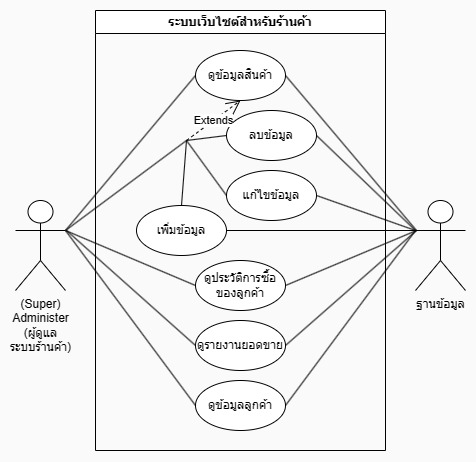
\includegraphics[scale=0.5]{pic/diagram/usecase-web.jpg}
  \end{center}

  \caption[Dataset generator]{Dataset generator}
  \label{fig:Website Application Use Case Diagram}
\end{figure}
\begin{figure}[h]
  \begin{center}

    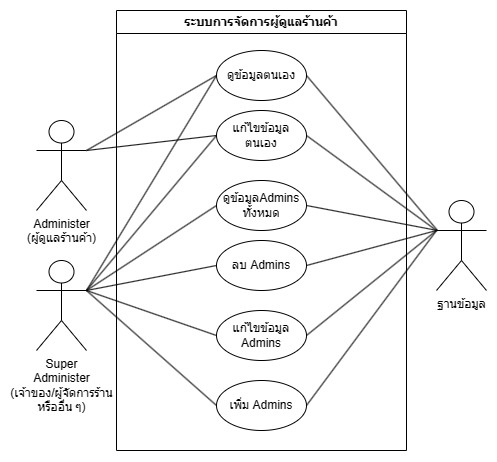
\includegraphics[scale=0.5]{pic/diagram/use-case-admin.jpg}
  \end{center}

  \caption[Dataset generator]{Dataset generator}
  \label{fig:Administer System Use Case Diagram}
\end{figure}

\begin{table}[htbp]
  \centering
  \caption{แสดงการอธิบายกรณีการใช้งานกรณีดูข้อมูลสินค้าของระบบเว็บไซต์สำหรับร้านค้า}
  \label{tab:example}
  \begin{tabularx}{\textwidth}{|p{3cm}|X|}
      \hline
      \multirow{1}{3cm}{Use Case ID:} & 1 \\
      \hline
      \multirow{1}{3cm}{Use Case Name:} & ดูข้อมูลสินค้า \\
      \hline
      \multirow{1}{3cm}{Actor:} & 1. ผู้ดูแลระบบร้านค้า  2. ฐานข้อมูล \\
      \hline
      \multirow{1}{3cm}{Pre-Condition:} & เข้าสู่ระบบ \\
      \hline
      \multirow{1}{3cm}{Post-Condition:} & แสดงข้อมูลสินค้าตามหมวดหมู่ พร้อมรายละเอียดทั้งหมด \\
      \hline
      \multirow{3}{3cm}{Event flow:} & 1. เข้าสู่ระบบ  \\ 
      & 2. กดเมนู Stock Manager \\ 
      \hline
      \multirow{1}{3cm}{Alternative flow:} & - \\
      \hline
  \end{tabularx}
\end{table}

\begin{table}[htbp]
  \centering
  \caption{แสดงการอธิบายกรณีการใช้งานกรณีลบข้อมูลของระบบเว็บไซต์สำหรับร้านค้า}
  \label{tab:example}
  \begin{tabularx}{\textwidth}{|p{3cm}|X|}
      \hline
      \multirow{1}{3cm}{Use Case ID:} & 2 \\
      \hline
      \multirow{1}{3cm}{Use Case Name:} & ลบข้อมูลสินค้า \\
      \hline
      \multirow{1}{3cm}{Actor:} & 1. ผู้ดูแลระบบร้านค้า  2. ฐานข้อมูล \\
      \hline
      \multirow{1}{3cm}{Pre-Condition:} & 1. เข้าสู่ระบบ 2. กดเมนู Stock Manager \\
      \hline
      \multirow{1}{3cm}{Post-Condition:} & ลบหมวดหมู่สินค้า และ/หรือสินค้าออกจากฐานข้อมูล \\
      \hline
      \multirow{3}{3cm}{Event flow:} & 1. กดเมนู Stock Manager  \\ & \textbf{กรณีที่ 1: ลบหมวดหมู่สินค้า} \\
      & 2. กดที่การ์ดหมวดหมู่สินค้า \\ & 3. แสดงปุ่มลบหมวดหมู่สินค้าในการ์ดหมวดหมู่นั้น ๆ \\
      & 4. กดลบหมวดหมู่สินค้า และกดยืนยัน \\ & 5. แสดงผลการลบหมวดหมู่สินค้าสำเร็จ \\
      & \textbf{กรณีที่ 2: ลบสินค้า} \\ & 2. กดที่การ์ดหมวดหมู่สินค้า \\
      & 3. แสดงปุ่มสินค้าทั้งหมดหมวดหมู่นั้น ๆ \\ & 4. กดที่การ์ดสินค้า เพื่อแสดงปุ่มลบสินค้า \\
      & 5. กดลบสินค้า และกดยืนยัน \\ & 6. แสดงผลการลบสินค้าสำเร็จ \\
      \hline
      \multirow{1}{3cm}{Alternative flow:} & - \\
      \hline
  \end{tabularx}
\end{table}

\begin{table}[htbp]
  \centering
  \caption{แสดงการอธิบายกรณีการใช้งานกรณีแก้ไขข้อมูลสินค้าของระบบเว็บไซต์สำหรับร้านค้า}
  \label{tab:example}
  \begin{tabularx}{\textwidth}{|p{3cm}|X|}
      \hline
      \multirow{1}{3cm}{Use Case ID:} & 3 \\
      \hline
      \multirow{1}{3cm}{Use Case Name:} & แก้ไขข้อมูลสินค้า \\
      \hline
      \multirow{1}{3cm}{Actor:} & 1. ผู้ดูแลระบบร้านค้า  2. ฐานข้อมูล \\
      \hline
      \multirow{1}{3cm}{Pre-Condition:} & 1. เข้าสู่ระบบ 2. กดเมนู Stock Manager \\
      \hline
      \multirow{1}{3cm}{Post-Condition:} & แก้ไขข้อมูลสินค้าบนฐานข้อมูล \\
      \hline
      \multirow{3}{3cm}{Event flow:} & 1. กดที่การ์ดหมวดมหมู่สินค้าที แล้วกดการ์ดสินค้าที่ต้องการ เพื่อแสดงปุ่มแก้ไขสินค้า  \\
      & 2. กดปุ่มแก้ไขสินค้า \\ & 3. แสดงหน้าต่างการแก้ไขข้อมูล พร้อมข้อมูลเดิม \\
      & 4. ผู้ดูแลระบบร้านค้ากรอกข้อมูลที่ต้องการแก้ไข และกดยืนยัน \\ & 5. แสดงผลการแก้ไขสินค้าสำเร็จ \\
      \hline
      \multirow{1}{3cm}{Alternative flow:} & - \\
      \hline
  \end{tabularx}
\end{table}

\begin{table}[htbp]
  \centering
  \caption{แสดงการอธิบายกรณีการใช้งานกรณีเพิ่มข้อมูลสินค้าของระบบเว็บไซต์สำหรับร้านค้า}
  \label{tab:example}
  \begin{tabularx}{\textwidth}{|p{3cm}|X|}
      \hline
      \multirow{1}{3cm}{Use Case ID:} & 4 \\
      \hline
      \multirow{1}{3cm}{Use Case Name:} & เพิ่มข้อมูลข้อมูลสินค้า \\
      \hline
      \multirow{1}{3cm}{Actor:} & 1. ผู้ดูแลระบบร้านค้า  2. ฐานข้อมูล \\
      \hline
      \multirow{1}{3cm}{Pre-Condition:} & 1. เข้าสู่ระบบ 2. กดเมนู Stock Manager \\
      \hline
      \multirow{1}{3cm}{Post-Condition:} & เพิ่มข้อมูลสินค้าบนฐานข้อมูล \\
      \hline
      \multirow{3}{3cm}{Event flow:} & 1. กดเมนู Stock Manager  \\ & \textbf{กรณีที่ 1: เพิ่มหมวดหมู่สินค้า} \\
      & 2. กดปุ่มหมวดหมู่สินค้า \\ & 3. กรอกข้อมูลหมวดหมู่สินค้าใหม่ และกดยืนยัน \\
      & 5. แสดงผลการเพิ่มหมวดหมู่สินค้าสำเร็จ \\
      & \textbf{กรณีที่ 2: ลบสินค้า} \\ & 2. กดที่การ์ดหมวดหมู่สินค้า \\
      & 3. แสดงปุ่มเพิ่มสินค้าในหมวดหมู่นั้น ๆ \\ & 4. กรอกข้อมูลสินค้าใหม่ และกดยืนยัน \\
      & 5. แสดงผลการเพิ่มสินค้าสำเร็จ \\
      \hline
      \multirow{1}{3cm}{Alternative flow:} & - \\
      \hline
  \end{tabularx}
\end{table}

\begin{table}[htbp]
  \centering
  \caption{แสดงการอธิบายกรณีการใช้งานกรณีดูประวัติการซื้อของลูกค้าบนระบบเว็บไซต์สำหรับร้านค้า}
  \label{tab:example}
  \begin{tabularx}{\textwidth}{|p{3cm}|X|}
      \hline
      \multirow{1}{3cm}{Use Case ID:} & 5 \\
      \hline
      \multirow{1}{3cm}{Use Case Name:} & ดูประวัติการซื้อของลูกค้า \\
      \hline
      \multirow{1}{3cm}{Actor:} & 1. ผู้ดูแลระบบร้านค้า  2. ฐานข้อมูล \\
      \hline
      \multirow{1}{3cm}{Pre-Condition:} & เข้าสู่ระบบ \\
      \hline
      \multirow{1}{3cm}{Post-Condition:} & ผู้ดูแลระบบร้านค้ารับรู้ประวัติการซื้อของลูกค้า \\
      \hline
      \multirow{3}{3cm}{Event flow:} & 1. กดเมนู Purchase History  \\ 
      & 2. แสดงรายการการซื้อของลูกค้าแต่ละครั้งในรูปแบบการ์ด ประกอบไปด้วยชื่อ วัน และเวลาที่ซื้อ พร้อมรายการสินค้าที่ซื้อ และจำนวนเงินที่จ่าย \\
      \hline
      \multirow{1}{3cm}{Alternative flow:} & 2. ไม่มีรายการแสดงหากยังไม่มีลูกค้าซื้อสินค้าผ่านระบบแอปพลิเคชันบนโทรศัพท์มือถือ \\
      \hline
  \end{tabularx}
\end{table}

\begin{table}[htbp]
  \centering
  \caption{แสดงการอธิบายกรณีดูรายงานยอดขายสินค้าของระบบเว็บไซต์สำหรับร้านค้า}
  \label{tab:example}
  \begin{tabularx}{\textwidth}{|p{3cm}|X|}
      \hline
      \multirow{1}{3cm}{Use Case ID:} & 6 \\
      \hline
      \multirow{1}{3cm}{Use Case Name:} & ดูรายงานยอดขายสินค้า \\
      \hline
      \multirow{1}{3cm}{Actor:} & 1. ผู้ดูแลระบบร้านค้า  2. ฐานข้อมูล \\
      \hline
      \multirow{1}{3cm}{Pre-Condition:} & เข้าสู่ระบบ \\
      \hline
      \multirow{1}{3cm}{Post-Condition:} & ผู้ดูแลระบบร้านค้าทราบยอดขายโดยรวมของร้านตามที่ต้องการของ \\
      \hline
      \multirow{3}{3cm}{Event flow:} & 1. กดเมนู Selling Report  \\ 
      & 2. แสดงข้อมูลยอดขายของวันที่ปัจจุบันผ่านการ์ดข้อมูล แผนภูมิ และตาราง ในโหมดรายวัน ตามสินค้าทั้งหมด \\
      & \textbf{กรณีที่ 1:} \\ & 3. กดเลือกวันที่ที่ต้องการ \\
      & \textbf{กรณีที่ 2:} \\ & 3. กดเลือกแสดงตามรายวัน/สัปดาห์/เดือน/ปี \\
      & \textbf{กรณีที่ 3:} \\ & 3. กดเลือกแสดงตามหมวดหมู่สินค้า หรือสินค้าทั้งหมด \\
      & 4. แสดงข้อมูลยอดขายผ่านการ์ดข้อมูล แผนภูมิ และตาราง ตามตัวเลือกที่เลือกในข้อ 3 \\
      \hline
      \multirow{1}{3cm}{Alternative flow:} & 2. และ 4. แสดงไม่มีข้อมูลหากไม่มีประวัติการซื้อสินค้าในวันที่ที่เลือกบนฐานข้อมูล \\
      \hline
  \end{tabularx}
\end{table}

\begin{table}[htbp]
  \centering
  \caption{แสดงการอธิบายกรณีการใช้งานกรณีดูข้อมูลลูกค้าบนระบบเว็บไซต์สำหรับร้านค้า}
  \label{tab:example}
  \begin{tabularx}{\textwidth}{|p{3cm}|X|}
      \hline
      \multirow{1}{3cm}{Use Case ID:} & 7 \\
      \hline
      \multirow{1}{3cm}{Use Case Name:} & ดูข้อมูลลูกค้า \\
      \hline
      \multirow{1}{3cm}{Actor:} & 1. ผู้ดูแลระบบร้านค้า  2. ฐานข้อมูล \\
      \hline
      \multirow{1}{3cm}{Pre-Condition:} & เข้าสู่ระบบ \\
      \hline
      \multirow{1}{3cm}{Post-Condition:} & ผู้ดูแลระบบร้านค้ารับรู้ข้อมูลของลูกค้า \\
      \hline
      \multirow{3}{3cm}{Event flow:} & 1. กดเมนู Customers  \\ 
      & 2. แสดงข้อมูลของลูกค้าทั้งหมดผ่านตาราง และการ์ดข้อมูล ได้แก่จำนวนลูกค้าทั้งหมด จำนวนลูกค้าที่ลงทะเบียนใหม่ใน 7 วันที่ผ่านมา และข้อมูลของลูกค้าแต่ละคน \\
      \hline
      \multirow{1}{3cm}{Alternative flow:} & 2. ไม่มีรายการแสดงหากยังไม่มีลูกค้าลงทะเบียนผ่านระบบแอปพลิเคชันบนโทรศัพท์มือถือ \\
      \hline
  \end{tabularx}
\end{table}

\section{การจัดทำฐานข้อมูล}
ในส่วนของการจัดทำฐานข้อมูล ได้เลือกใช้ Supabase ซึ่งเป็นเซอร์วิสสำหรับการสร้างและจัดการฐานข้อมูล (Database) แบบ Open Source ที่ให้บริการในรูปแบบฮอสต์ (hosted) ซึ่งเป็นเซอร์วิสที่ให้บริการแบบคลาวด์ (cloud services) ประกอบด้วยฐานข้อมูลแบบ PostgreSQL และบริการอื่น ๆ เช่น Authentication, Realtime Database, Storage และ APIs ทำให้สามารถจัดการข้อมูลได้สะดวก และมีประสิทธิภาพ โดยมีการเก็บ Database Schema เพื่อครอบคลุมการเก็บข้อมูลที่ใช้ในฝั่งแอปพลิเคชันสำหรับโทรศัพท์มือถือ และเว็บไซต์สำหรับร้านค้า แสดงได้ดังนี้
\ref{fig:Database Schema}

\begin{figure}[h]
  \begin{center}

    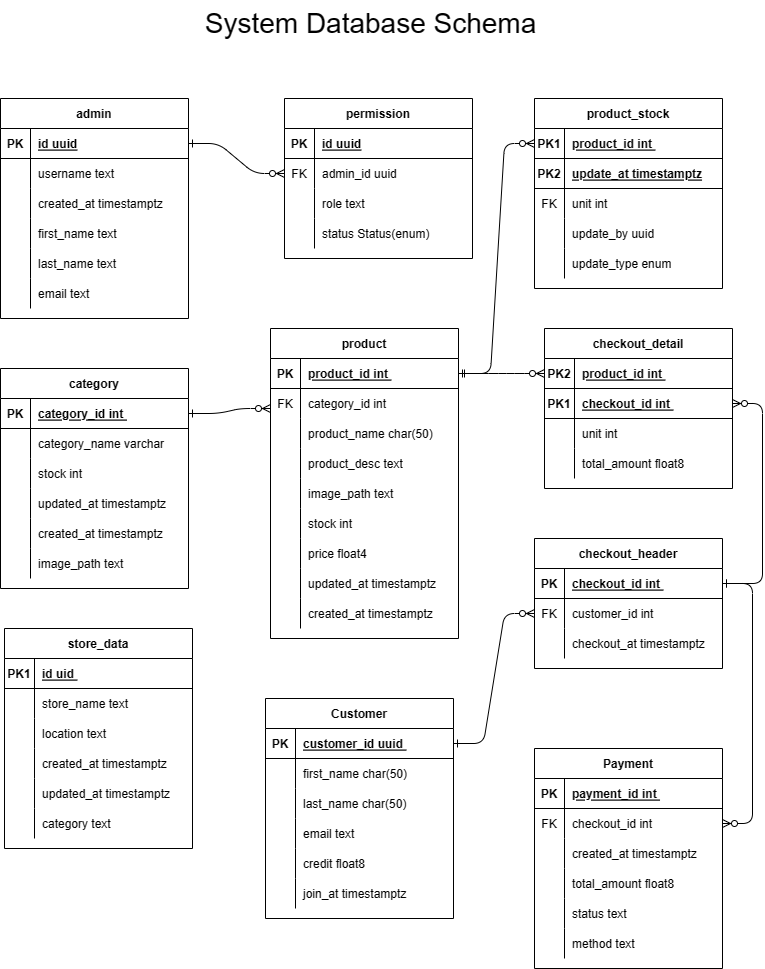
\includegraphics[scale=0.5]{pic/database.png}
  \end{center}

  \caption[System Database Schema]{System Database Schema}
  \label{fig:Database Schema}
\end{figure}

\begin{enumerate}
  \item Admin: เก็บข้อมูลของแอดมิน ซึ่งเป็นผู้ที่สามารถเข้าถึงและแก้ไขข้อมูลร้านค้าได้ โดยในร้านหนึ่ง ๆสามารถมีแอดมินได้มากกว่าหนึ่งคน ซึ่งจะเก็บข้อมูลชื่อจริง รหัสผ่าน ที่อยู่อีเมล์ และรูปภาพของแอดมิน โดยมี Primary key เป็นชื่อผู้ใช้ หรือ username
  \item Permission: เก็บสถานะของแอดมิน ได้แก่ Administers และ Super Administers Foreign key จากตาราง admin คือ admin\_id
  \item Product: เก็บข้อมูลขอฃสินค้าแต่ละชนิดได้แก่ ชื่อสินค้า รูปสินค้า จำนวนสินค้าในคลัง ราคาสินค้า คำอธิบายสินค้า และหมวดหมู่สินค้าซึ่งเป็น Foreign key จากตาราง category และมี Primary key คือ รหัสหรือ product\_id
  \item Category: เก็บข้อมูลของหมวดหมู่สินค้า ซึ่งประกอบไปด้วยชื่อ และคำอธิบายของหมวดหมู่สินค้า โดยมี Primary key คือ รหัสหมวดหมู่สินค้า หรือ category\_id
  \item Checkout\_header: เก็บข้อมูลคำสั่งซื้อสินค้าทั้งหมดของร้านค้า ซึ่งประกอบไปด้วยวันที่ และเวลาที่สั่งซื้อ ยอดขายจากคำสั่งซื้อ หมายเลขระบุตัวตนลูกค้าหรือ customer\_id จากตาราง customer และรหัสชำระเงิน หรือ payment\_id  จากตาราง Payment ซึ่งมี Primary key คือ หมายเลขระบุคำสั่งซื้อ หรือ checkout\_id
  \item Checkout\_detail: เก็บข้อมูลสินค้าที่ถูกซื้อของแต่ละคำสั่งซื้อ โดยเก็บ Foreign key เป็นหมายเลขระบุคำสั่งซื้อ หรือ checkout\_id จากตาราง checkout\_header และรหัสสินค้า หรือ product\_id จากตาราง product ควบคู่กันเป็น Primary key และเก็บข้อมูลอื่น ๆ ได้แก่ จำนวนสินค้าที่สั่งซื้อ และจำนวนเงินที่จ่ายทั้งหมด
  \item Customer: เก็บข้อมูลลูกค้าของร้านค้า โดยเก็บชื่อ username ของลูกค้า และมี Primary key คือ หมายเลขระบุตัวตนลูกค้าหรือ customer\_id
  \item Product\ stock: เก็บข้อมูลการเปลี่ยนแปลงจำนวนสินค้าในคลัง โดยเก็บ Foreign key เป็นหมายเลขระบุสินค้า หรือ product\_id จากตาราง Product และจำนวนสินค้าที่เพิ่ม หรือลด มี Primary key คือ ชื่อผู้ใช้งานแอดมินผู้เปลี่ยนจำนวนสินค้าในคลัง หรือ username จากตาราง Admin ควบคู่กับวันที่และเวลาที่ทำการเปลี่ยน หรือ timestamp
  \item Payment: เก็บข้อมูลการชำระเงิน ซึ่งประกอบไปด้วยประเภทการชำระเงิน วันที่ และเวลาของการชำระเงิน และสถานะการชำระเงิน และเก็บ Foreign key เป็นหมายเลขระบุตัวตนลูกค้า หรือ customer\_id  มี Primary key คือ รหัสชำระเงิน หรือ payment\_id
  \item Store data: เก็บข้อมูลของร้านค้า ได้แก่ ชื่อ สถานที่ตั้ง และ ประเภทร้านค้า

\end{enumerate}
เนื่องจาก Supabase นั้นสนับสนุนการใช้งาน PostgreSQL จึงได้มีการออกแบบฟังก์ชัน PostgreSQL เพื่อดำเนินการต่าง ๆ กับข้อมูลในฐานข้อมูลที่ซับซ้อน และต้องการการประมวลผลต่าง ๆ เช่น การค้นหาข้อมูล (query), การเพิ่มข้อมูล (insert), การปรับปรุงข้อมูล (update), และการลบข้อมูล (delete) ซึ่งได้ทำทั้งหมด 23 ฟังก์ชัน


% \section{การทดสอบการทำงานของซอร์ฟแวร์}
% การทดสอบการทำงานของระบบ สามารถแบ่งเป็นขั้นตอนดังนี้
% \subsection{Unit testing}
% การทดสอบความถูกต้องของการทำงานในแต่ละฟังก์ชันหลักของระบบแยกกัน โดยยังไม่รวมแต่ละ Component เข้าด้วยกัน ซึ่งได้แก่
% \begin{enumerate}
%   \item Classification system
%   \item Website dashboard
%   \item Mobile Application
% \end{enumerate}

% \subsection{Integration testing}
% การทดสอบการทำงานเมื่อรวมระบบย่อยทั้งหมดเข้าด้วยกัน โดยหลัก ๆ
% จะทดสอบในเรื่อง API ว่ามีการรับส่งข้อมูลดุถูกต้องหรือไม่ และทำงานโดยรวมได้ถูกต้องทั้งหมดหรือไม่
% \subsection{System testing}
% การทดสอบระบบซึ่งแต่ละโมดูลข้างต้นจะถูกรวม และทดสอบเป็นกลุ่ม
% เพื่อประเมินความสอดคล้องของระบบว่าทำงานได้ตามที่กำหนดไว้หรือไม่
% \subsection{Acceptance testing}
% การทดสอบระบบโดยดูภาพรวมของการทำงาน ว่ามีการตอบสนองความต้องการของผู้ใช้ทั้งในส่วนของฟังก์ชันการทำงาน
% และประสิทธิภาพการทำงาน ว่าสอดคล้องกับลักษณะของความต้องการของซอฟต์แวร์หรือไม่
% โดยใช้การทดสอบแบบ Functional testing (Black box testing)



% \subsection{The Black Kitten}
% One thing was certain, that the WHITE kitten had had nothing to
% do with it:---it was the black kitten's fault entirely



% ~\cite{aiw}. 




%  For the
% white kitten had been having its face washed by the old cat for
% the last quarter of an hour (and bearing it pretty well,
% considering); so you see that it COULDN'T have had any hand in
% the mischief.

%   The way Dinah washed her children's faces was this:  first she
% held the poor thing down by its ear with one paw, and then with
% the other paw she rubbed its face all over, the wrong way,
% beginning at the nose:  and just now, as I said, she was hard at
% work on the white kitten, which was lying quite still and trying
% to purr---no doubt feeling that it was all meant for its good.

%   But the black kitten had been finished with earlier in the
% afternoon, and so, while Alice was sitting curled up in a corner
% of the great arm-chair, half talking to herself and half asleep,
% the kitten had been having a grand game of romps with the ball of
% worsted Alice had been trying to wind up, and had been rolling it
% up and down till it had all come undone again; and there it was,
% spread over the hearth-rug, all knots and tangles, with the
% kitten running after its own tail in the middle.

% \subsection{The Reproach}

